\documentclass[a4paper,12pt]{book}
% Paquetes de la ams
\usepackage{amsmath,amsthm,amssymb,amsfonts}
% Codificacion UTF-8
\usepackage[utf8]{inputenc}
% Tablas e imagenes en espaniol
\usepackage[spanish,es-tabla]{babel}
% Mejores graficos
\usepackage{graphicx}
% tablas mas lindas
\usepackage{booktabs}
% Links a urls
\usepackage{url}
% Linkear referencias en pdfs
\usepackage{hyperref}
% Texto mas lindo para los pie de figura
\usepackage[margin=10pt,font=small,labelfont=bf, labelsep=endash]{caption}

% Citas
\usepackage[backend=biber,style=ieee]{biblatex}
\addbibresource{biblio.bib}

% Codigo
\usepackage{listings}

% Dir tree
\usepackage{dirtree}

% Pagina en blanco cuando ha
\usepackage{emptypage}

\definecolor{A11}{HTML}{B2DF8A}
\definecolor{A12}{HTML}{33A02C}
\definecolor{A23}{HTML}{FDBF6F}
\definecolor{A24}{HTML}{FF7F00}
\definecolor{B15}{HTML}{FB9A99}
\definecolor{B16}{HTML}{E31A1C}
\definecolor{B27}{HTML}{A6CEE3}
\definecolor{B28}{HTML}{1F78B4}

% Ejemplos, observaciones y teorema
\theoremstyle{definition}
\newtheorem{exa}{Ejemplo}[section]
\newtheorem*{obs}{Observación}
\newtheorem{que}{Pregunta}[section]
\newtheorem{dex}{Definicion}[section]


\graphicspath{{./figs/}}

\title{Curso Nivel 2a}
\author{Francisco Nemiña}
\begin{document}
\maketitle
\titlepage
\chapter{Firmas espectrales}
El objetivo de esta clase es doble. Por un lado familiarizarse con el entorno gráfico del \emph{Sentinel Aplication Toolbox (SNAP)}. Por otro comprender el concepto de firma espectral por medio del estudio de sus valores dentro de la imagen.

\section{Interfaz gráfica del SNAP}

Descomprima los archivos decargados que se denominan \path{material.tar.gz}. Abra el programa SNAP, allí encontra la interfaz gráfica del usuario (Figura \ref{fig:int})

\begin{figure}[h]
    \centering
    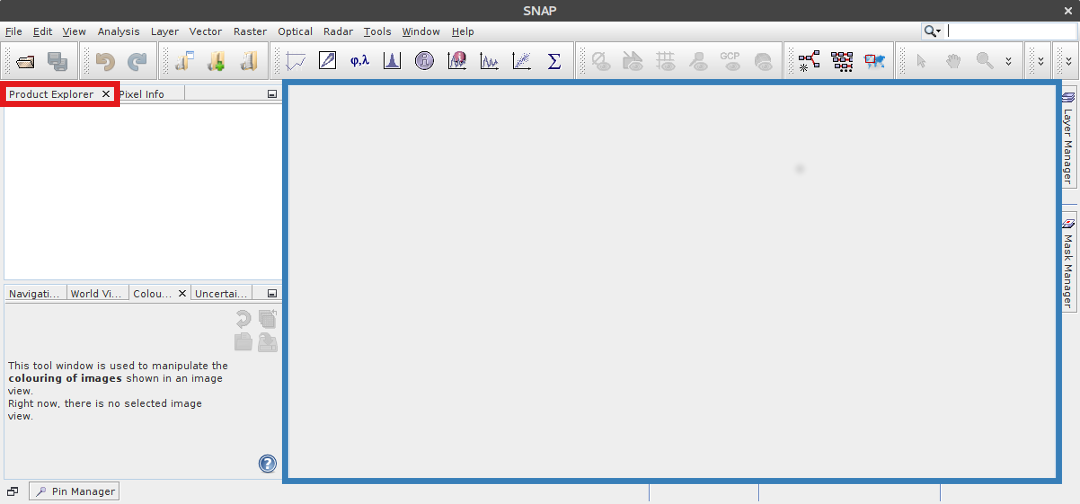
\includegraphics{fig:int.png}
    \caption{Interfáz gráfica del usuario. El árbol de capas y el area de visualización se encuentran siempre al abrir el programa.}
    \label{fig:int}
\end{figure}

En el menú principal, seleccione \emph{Open product...} o presione [BOTON ABRIR] y dentro de la carpeta \path{material/raster_data}, seleccione \path{S2A_MSIL2A_20170720.dim}.

La cobertura que aparecerá en el árbol de capas es más completa que la típica cobertura raster que se encuentra en la mayoría de los software.

Haciendo click a la derecha de la misma se desplegará un árbol que incluye las opciones:
\dirtree{%
    .1 [1] S2\_MSIL2A\_20170702.
    .2 Metadaata.
    .2 Index Codings.
    .2 Vector Data.
    .2 Bands.
    .2 Masks.
}

De esta cobertura se destaca:

\begin{itemize}
    \item \emph{[1] S2\_MSIL2A\_20170702}: El número de elemento, entre corchetes, y el nombre de la imagen.
    \item \emph{Metadata}: Los metadatos asociados a la imagen y su historia de procesamiento.
    \item \emph{Index Codings}: Los valores de referencia de como interpretar dentro de la imagen y las máscaras distintos valores.
    \item \emph{Vector data}: Las capas vectoriales que se encuetran asociadas a la imagen.
    \item \emph{Bands}: Las bandas de la imagen y las operaciones de álgebra que bandas que operemos sobre ellas.
    \item \emph{Masks}: Las mascaras que sean incluidas en la imagen o las que creemos.
\end{itemize}

Si despliega la carpeta \emph{Bands} dentro de la imagen abierta pueded mostrar cualquiera de las bandas haciendo doble click sobre ella.

\begin{que}
    ¿Cuantas bandas encuentra dentro del archivo? ¿A que longitudes de onda corresponden? ¿En que zonas del espectro está el mayor número de bandas?
\end{que}

\section{Combinaciones espectrales}

Para realizar combinaciones espectrales con la imagen abierta haga click derecho sobre el nombre en el \emph{Product Explorer} y luego en \emph{Open RGB image windows.}. Se desplegará una nueva ventana (Figura \ref{fig:RGB}) que nos permitirá elegir la combinación de bandas.

\begin{figure}[h]
    \centering
    %\includegraphics{}
    \caption{Ventana para elegir la combinación de bandas. Puede seleccionarla eligiendo una banda para cada canal del monitor ,\emph{Red, Green, Blue} o puede utilizar una preseleccionada del menú \emph{Profile}}
    \label{fig:RGB}
\end{figure}

Por defecto elegirá la combinación de bandas que utiliza las bandas 4, 3 y 2 de Sentinel 2 y la desplegará haciendo click en OK (Figura \ref{fig:RVA}).

\begin{figure}[h]
    \centering
    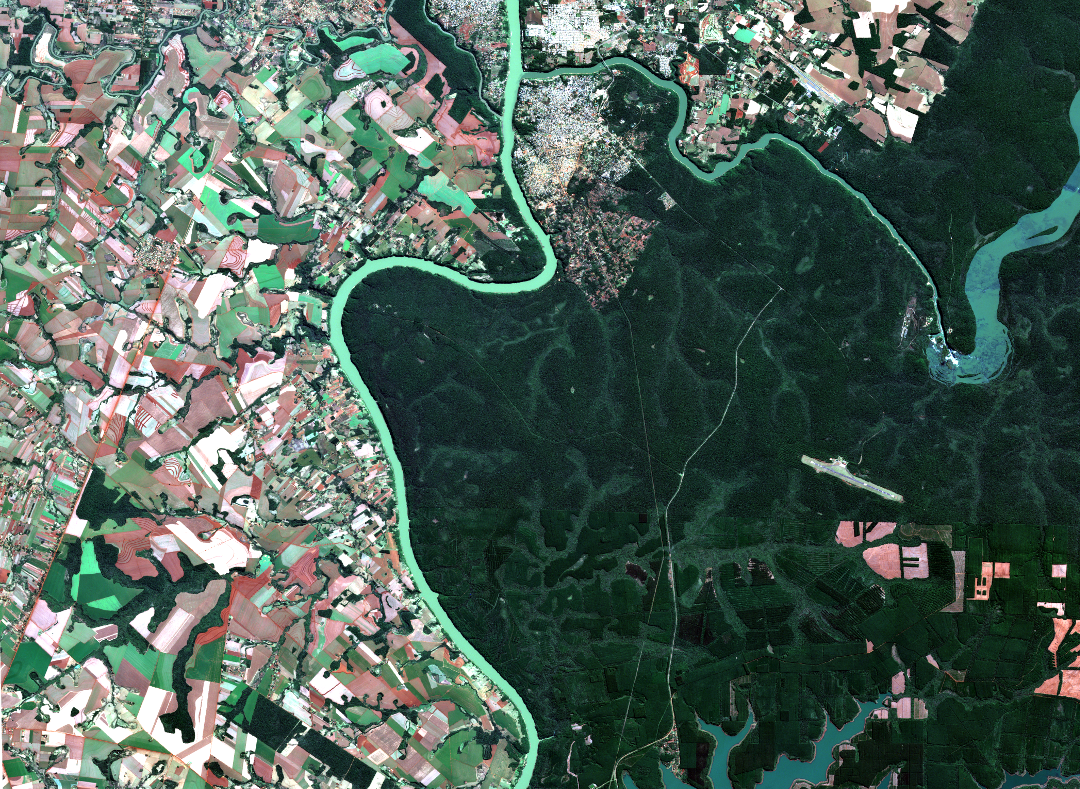
\includegraphics{fig:RVA.png}
    \caption{Imagen en combinación de colores de color real.}
    \label{fig:RVA}
\end{figure}

\begin{que}
    ¿A que longitudes de onda pertenecen cada una de estas bandas? ¿Con que colores las identificamos?
\end{que}

Muevase dentro de la imagen utilizando las herramientas de navegación y zoom (Figura \ref{fig:NAV})

\begin{figure}[h]
    %\includegraphics{}
    \caption{Herramientass de navegación.}
    \label{fig:NAV}
\end{figure}

Explore la imagen desplegada en esta combinación de color.

\begin{que}
    ¿Observa diferencias en los colores de los distintos cuerpos de agua? ¿Y en los colores de la selva y las forestaciones? ¿Que le dice la diferencia observada sobre la firma espectral de los distintos cuerpos de agua? ¿Será posible separar espectralmente las forestaciones de la selva utilizando unicamente la zona visible del espectro electromagnetico?
\end{que}

Seleccione ahora la combinacion de color RGB \emph{Sentinel 2 MSI False-color Infrarred} que incluye a una banda del infrarrojo cercano y dos del visible (Figura \ref{fig:NRG}). Explore la imagen desplegada en esta combinación de color.

\begin{figure}[h]
    \centering
    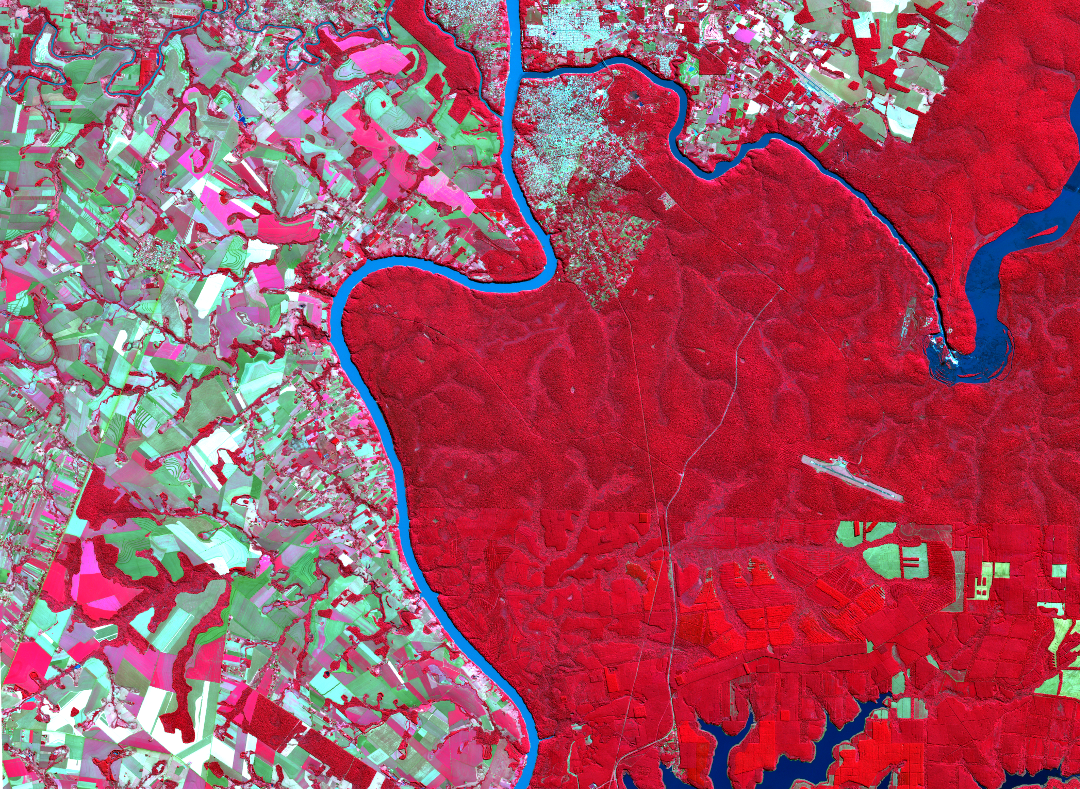
\includegraphics{fig:NRG.png}
    \caption{Imagen en combinación de colores infrarrojo color.}
    \label{fig:NRG}
\end{figure}

\begin{que}
    ¿Observa diferencias en los colores de los distintos cuerpos de agua? ¿Pueded distinguir más o menos detalles dentro de los mismos que con la combinación de color real? ¿Y en los colores de la selva y las forestaciones? ¿Será posible separar espectralmente las forestaciones de la selva utilizando unicamente la zona del espectro visible del visible y el infrarrojo cercano? ¿Considerando la relación entre la reflectancia en el NIR y los parametros biofísicos, que pueded predecir sobre el porcentaje de cobertura de la selva y las forestaciones?
\end{que}

Seleccione ahora la combinacion de color RGB \emph{Sentinel 2 MSI Healthy Vegetation} que incluye a una banda del infrarrojo cercano, una del infrarrojo medio y una del visible (Figura \ref{fig:SNR}). Explore la imagen desplegada en esta combinación de color.

\begin{figure}[h]
    \centering
    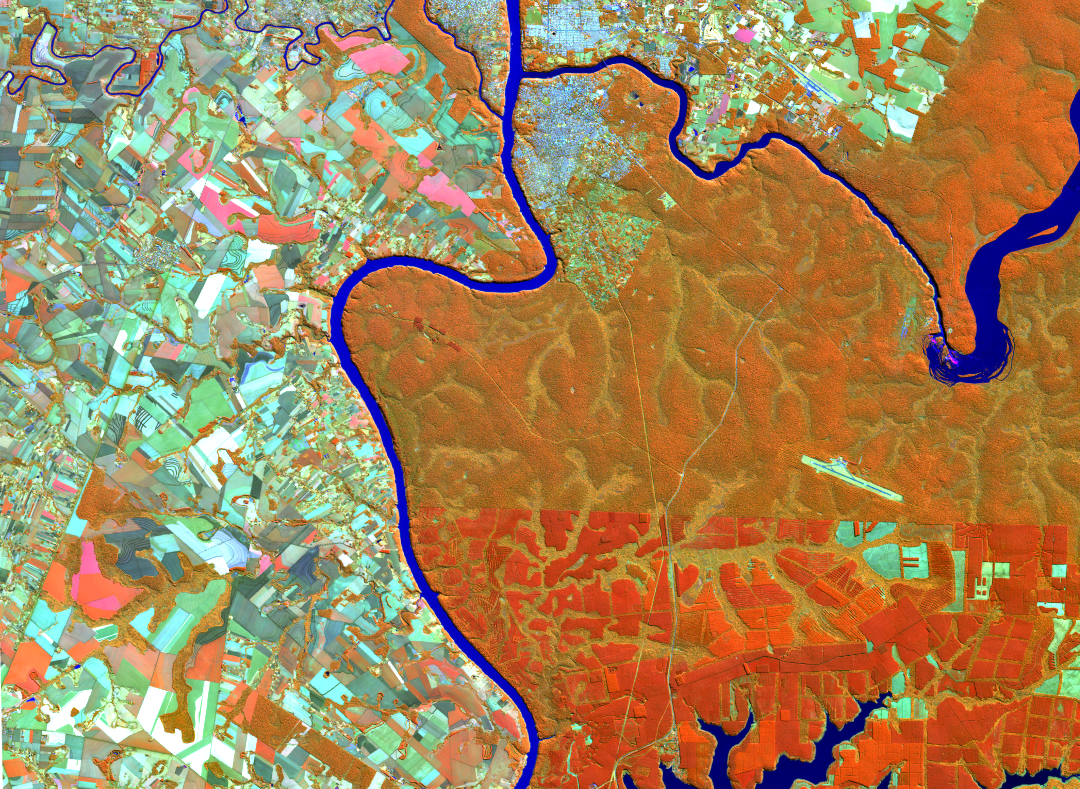
\includegraphics{fig:SNR.png}
    \caption{Imagen en combinación de colores falso color compuesto.}
    \label{fig:SNR}
\end{figure}


\begin{que}
    ¿Es posible separar a las forestaciones de la selva en esta combinación de bandas? ¿Cual es la caracteristica biofísica que mayor cambia entre la selva y las forestaciones? ¿Es posible distinguir grandes diferencias entre los cuerpos de agua dentro de la imagen en esta combinación de bandas?
\end{que}

\begin{que}
    ¿Que combinación de bandas le aporta más información sobre la vegetación? ¿Puede explicar esto desde el punto de vista de la firma espectral de la vegetación, sus variaciones en cada zona y las propiedades biofísicas de esta? ¿Que combinación de bandas le aporta más información sobre los cuerpos de agua?
\end{que}

\section{Firmas espectrales}

La herramienta \emph{Spectrum view} permite mostrar y extraer los valores de un píxel en función de la longitud de onda (Figura \ref{fig:sps}). Una vez extraidos estos pueden ser mostrados en pantalla como gráfico de lineas o guardados en un archivo de texto.

\begin{figure}
    %\includegraphics{/path/to/figure}
    \caption{Herraamienta \emph{Spectrum view} que permite mostrar lass firmas espectrales de distintos píxeles de la imagen.}
    \label{fig:sps}
\end{figure}

Despliegue la imagen \path{S2A_MSIL2A_20170720.dim} en una combinación de bandas conveniente para identificar distintas coberturas de vegetación. Luego hage click en la herramienta \emph{Spectrum view} y muevase dentro de la imagen para observar las firmas espectrales de las distintas coberturas.

\begin{que}
    ¿Cómo es la la firma espectral de la vegetación para las zonas de la selva que parecen hallarse más altas? ¿Y para las zonas de forestación? ¿Que pasa con la firma espectral en las distinas zonas de la ciudad de Puerto Iguazu?
\end{que}

Es posible agregar \emph{Pins} a la imagen y utilizarlo para mostrar la firma espectral sobre estos puntos. Para hacerlo seleccione la herramienta \emph{Pin placement tool} de la barra de herramienta y haga click sobre el Rio Iguazú. Observará que un pequeño pin aparece en este lugar (Figura \ref{fig:pin}).

\begin{figure}
    %\includegraphics{/path/to/figure}
    \caption{Pin sobre un píxel en la imagen.}
    \label{fig:pin}
\end{figure}

Utilice la herramienta \emph{Pin placement tool} para ubicar pines en distintas zonas de la imagen. Incluya al menos dos zonas de la selva cualitativamente ditintas, una zona de forestación y al menos un pin en el embalce Urugua-I, uno en el Rio Parana y otro en el Iguazu.

Haciendo click en \emph{Pin manager} se desplegará una nueva ventana  con propiedades de los pins. Puede observar en ella el pixel sobre el que se encuentra, su latitud y longitud, el color del que se muestraa y la etiqueta \footnote{Label} que se le asigna. Asgine a cada pin una etiqueta y color diferenciado (Figura \ref{fig:pmg}).

\begin{figure}
    %\includegraphics{/path/to/figure}
    \caption{Ping manager}
    \label{fig:pmg}
\end{figure}

Una vez creados los pins es posibles mostrar la firma espectral de alguno o todos ellos. Abra para esto la herramienta \emph{Spectrum view} y seleccione las opciones: \emph{Show spectra for all pins}, para mostrar la firma espectral de todos los pins, o \emph{Show spectra for selected pins}, para mostra la firma espectral de los pines seleccionados (Figura \ref{fig:spn}).

\begin{figure}
    %\includegraphics{/path/to/figure}
    \caption{Ping manager}
    \label{fig:spn}
\end{figure}

Es posible también cambiar la escala con la que se muestra la la firma espectral haciendo click derecho sobre ella y eligiendo entre las opciones: \emph{Zoom in}, \emph{Zoom out} y \emph{Auto-range}.

Es además posible exportar las mediciones de la firma espectral. Por un lado puede guardar el gráfico haciendo click derecho sobre el y eligiendo la opción \emph{Save as...}. Por otro, puede exportar los valores de reflectancia de la firma espectral haciendo click en el botón \emph{Export spectra to text file}.

Compare las firmas espectrales de las zonas de forestación y selva paranense (Figura \ref{fig:svg}).

\begin{figure}
    %\includegraphics{/path/to/figure}
    \caption{Firmas espectrales de vegetación.}
    \label{fig:svg}
\end{figure}

\begin{que}
    ¿En que zonas del espectro son más similares las firmas de Selva Alta y Forestación? ¿En que zonas del espectro son más distintas las tres firmasa espectrales? ¿Que le permite decir esto sobre el contenido de contenido de relativo de pigmentos de las tres coberturas? ¿Y sobre el contenido relativo de humedad en la vegetación? ¿Que suposición está realizando al comparar las tres firmas?
\end{que}

Compare las firmas espectrales del rio Parana y el rio Iguazu cerca de la zona donde se juntan.

\begin{que}
    ¿En que zona del espectro electromagnético son más distintass las firmas espectrales? ¿A que se debe esta diferencia? ¿Que le dice sobre la combinación de bandas que más nos permite distinguir propiedades en los cuerpos de agua? ¿Cual de los dos rios parece tener mayor contenido de sedimento?
\end{que}

\section{Evaluación}

\begin{que}
    ¿Que combinación de bandas le permite distinguir más detalles sobre la vegetación?
\end{que}

\begin{que}
    ¿Que zona del espectro electromagnetico corresponde a [pigmentos,cobertura foliar,contenido de humedad] en la vegetacion?
\end{que}

\begin{que}
    ¿Cual de los tres cuerpos de agua presenta mayor contenido de sedimentos?
\end{que}

\end{document}
